% vim:spelllang=ru,en
\documentclass[simple,14pt,utf8,russian]{eskdtext}
\usepackage{eskddstu}
\ESKDtitle{{\small }}
\ESKDdocName{Пояснительная записка.}
\ESKDsignature{Экспертная система рекомендации литературы}
\ESKDauthor{Погода~М.\,В.}
\ESKDchecker{Голуб~А.\,Т.}
\ESKDgroup{{\scriptsize НТУУ <<КПИ>>, ФПМ, КМ-31м}}
\ESKDapprovedBy{{\scriptsize Молчанов~А.\,А.}}
\renewcommand{\ESKDfontShape}{\upshape}

\usepackage{cmap} % чтобы работал поиск по PDF
\usepackage[utf8]{inputenc}
% \usepackage[english,russian]{babel}
\usepackage[T2A]{fontenc}
% \usepackage{concrete}
\usepackage{pscyr}

% \usepackage[pdftex]{graphicx}
\usepackage{subfig}

\pdfcompresslevel=9 % сжимать PDF
% \usepackage{pdflscape} % для возможности альбомного размещения некоторых страниц
\usepackage{lscape}
\usepackage[pdftex]{hyperref}
% настройка ссылок в оглавлении для pdf формата
\hypersetup{unicode=true,
    pdftitle={Курсовой проект},
    pdfauthor={Погода Михаил},
    pdfcreator={pdflatex},
    pdfsubject={},
    pdfborder    = {0 0 0},
    bookmarksopen,
    bookmarksnumbered,
    bookmarksopenlevel = 2,
    pdfkeywords={},
    colorlinks=true, % установка цвета ссылок в оглавлении
    citecolor=black,
    filecolor=black,
    linkcolor=black,
    urlcolor=blue
}

\usepackage{amsmath}
\usepackage{amssymb}

\usepackage{listings}
\lstloadlanguages{Python,C++}
\lstset{language=Python,frame=tb,basicstyle=\scriptsize,commentstyle=\itshape,extendedchars=false}

\usepackage{multicol}

\begin{document}
\ESKDthisStyle{empty}
\begin{titlepage}
    \begin{center}
        \MakeUppercase{Министерство образования и науки Украины}\\
        \MakeUppercase{Национальный технический университет Украины}\\
        \MakeUppercase{<<Киевский политехнический институт>>}\\
        \vspace*{2em}

        Факультет прикладной математики\\
        Кафедра прикладной математики

        \vfill

        \MakeUppercase{Экспертная система рекомендации для интернет"=магазина технической литературы}\\
        \vspace*{2em}

        Курсовой проект\\
        по дисциплине:\\
        <<Экспертные системы>>
    \end{center}

    \vfill
    \begin{minipage}{0.6\textwidth}
        Руководитель:\\
        Голуб~А.\,Т.\\
        Защищено с оценкой~\underline{\hspace{5em}}
    \end{minipage}
    \hfill\begin{minipage}{0.3\textwidth}
        Выполнил студент\\
        группы КМ-31м\\
        Погода~М.\,В.
    \end{minipage}

    \vfill
    \begin{center}
        Киев\\
        2014
    \end{center}
\end{titlepage}

\ESKDthisStyle{formII}
\tableofcontents
\clearpage
\section*{ВВЕДЕНИЕ}
\addcontentsline{toc}{section}{Введение}
\label{chap:intro}
    Ни для кого не секрет, что двадцать первый век ---  эпоха информационного бума.
    По данным исследований компании IDC в 2011~г. общий объём информации, хранимой на всех существующих цифровых
    носителях информации, превысил $1.8 \times 10^{21}$~байт, а темпы ежегодного роста составляют порой $60\%$.
    Из-за такого стремительного возрастания количества информации люди перестают \textit{читать} и всё больше просто
    \textit{просматривают} материалы.~\cite{book1}
    Всё сложнее становится следить за всеми новыми интересными источниками информации, всё сложнее найти материалы,
    которые необходимо прочитать для изучения той или иной области.

    Особенно сильно это задевает область информационных технологий.
    Часть литературы по информационным технологиям устаревает очень быстро, часть остаётся актуальной всегда, часть
    занимает очень узкую нишу, часть же наоборот получает мировое признание.

    В любом случае, всё сложнее становится выбрать книгу по информационным технологиям, которая наиболее полно ответит
    интересам пользователя.
    Сложность также заключается в том, что человек, в особенности новичок, не всегда знает, что он хочет
    узнать/освоить в результате.~\cite{book2}

    Основным путём решения этой проблемы является расспрашивание более опытных знакомых, интересующихся той же
    тематикой; общение на форумах\dots

    В курсовом проекте рассматривается экспертная система, позволяющая рекомендовать техническую литературу на
    основании анкетирования человека.
    \clearpage
\section{Задание на проектирование}
\label{chap:task}
    Целью данного проекта является разрабатывание подхода, в основе которого лежит использование экспертной системы
    для рекомендации литературы по информационным технологиям.

    Объект исследования --- экспертные системы в контексте рекомендаций на основе анкетирования, модели представления
    знаний.

    Предмет исследования --- применение экспертных систем для рекомендации технической литературы по информационным
    технологиям.
    \clearpage
\section{Идентификация}
\label{chap:identitication}
    \subsection{Описание предметной и проблемной области}
    \label{sec:description}
    Предметная область проектируемой экспертной системы --- научная и учебная литература.

    В научной литературе фиксируются и обобщаются результаты научных исследований, а также их анализ.
    К научной литературе примыкают \textit{учебная} и \textit{научно"=популярная} литература.
    Учебная литература предназначена для подготовки специалистов в определённых областях знаний и профессий.
    Основной вид учебной литературы --- учебник и справочник.

    Научно"=популярная литература предназначена для распространения знания и ориентируется на неподготовленных в
    данной области науки читателей.
    Её цель ---  заинтересовать читателя и предоставить ему некоторое представление про достижения современной науки.

    Экспертная система разрабатывается в качестве расширения интернет"=магазина технической литературы.
    Основным идентификатором каждого наименования является адрес, по которому его можно приобрести.

    Главными функциями системы являются:
    \begin{itemize}
        \item анализ поведения пользователя;
        \item определение предпочтений пользователей на основе анкетирования, анализа их поведения;
        \item группирование пользователей по предпочтениям;
        \item рекомендация литературы согласно предпочтениям пользователя;
        \item добавление новых наименований.
    \end{itemize}
    \clearpage
\section{Концептуализация}
\label{chap:concept}
    \subsection{Разрабатывание основных принципов построения ЭС}
    \label{sec:principles}
        \subsubsection{Дерево решений}
        \label{ssec:tree}
            На рисунке~\ref{fig:tree} изображено дерево принятия решений, которое используется для начального
            анкетирования, если у пользователя отсутствует начальный список предпочтений.
        \subsubsection{Описание метода решения задачи}
        \label{ssec:method}
            Существующие на сегодня адаптивные системы рекомендаций формируют предпочтения пользователей за счёт их
            взаимодействия с системой, сохраняют эти предпочтения в профиле пользователя и используют их для
            формирования индивидуальных списков рекомендации.
            Целью такой организации является повышение качества обратной связи.~\cite{book3}

            Проектируемая экспертная система определяет, с кем заданный пользователь имеет наибольшую схожесть
            интересов и формирует из таких людей группу.
            Считая, что предпочтения пользователей группы соответствует предпочтениям пользователя, система
            осуществляет основанный на опыте группы поиск рекомендаций.
            Благодаря использованию такой модели поведения пользователей проектируемая система должна регулярно
            перестраивать группы пользователей.

            Для определения групп пользователей, имеющих схожие интересы, можно использовать методы кластеризации.
            Например, метод \textit{$k$ ближайших соседей}.
            Метод $k$ ближайших соседей --- метод автоматической классификации объектов.
            Основным принципом метода ближайших соседей является то, что объект присваивается тому классу, который
            является наиболее распространённым среди соседей данного элемента.~\cite{book5}

            Такой подход к кластеризации и поиска рекомендаций позволяет достигнуть цели за время,
            пропорциональное~$O(mn)$, где $m$ --- количество пользователей, $n$ --- количество разделов.~\cite{book4}

    \subsection{Выбор модели представления знаний}
    \label{sec:model}
        Для реализации базы знаний была использована модель фреймов.
        Эта модель позволяет описать данные в наиболее пригодном для разрабатываемой системы виде.

        Фрейм --- структура данных, описывающая некоторую стандартную ситуацию.
        Фрейм имеет фиксированную структуру (представляемую слотами и именем фрейма).
        Слоты содержат конкретные знания про атрибуты фрейма.
        Имя отражает суть фрейма как единого целого.

        В проектируемой экспертной системе использование фреймовой модели позволяет описывать вывод рекомендаций
        по-разному для разных групп пользователей.
        С помощью присоединённых процедур можно запрограммировать разные процедуры вывода.

        Механизм управления имеет следующий вид:
        \begin{enumerate}
            \item Сначала запускается одна из процедур некоторого фрейма (образец).
                Образец --- фрейм"=прототип, т.\,е. у него заданы только те слоты, которые описывают связи этого
                фрейма с другими.
            \item По запросу последовательно запускаются процедуры вывода других фреймов, таким образом формируется
                вывод списка рекомендаций.
        \end{enumerate}
    \subsection{Входные и выходные данные}
    \label{sec:io}
        Исходными данными для построения профиля пользователя и связанного с ним вектора являются история его покупок,
        а также начальные тематические приоритеты согласно предварительному анкетированию.
        Эти данные постоянно обновляются после каждого действия пользователя.
        Таким образом, вектор пользователя является активным.

        Используются следующие вектора интересов:
        \begin{itemize}
            \item Вектор просмотренной литературы $\vec{s}$.
                Формируется на основании истории покупок/закладок пользователя литературы одного подраздела.
                Каждая координата этого вектора характеризует частоту покупок/закладок соответствующего раздела.
            \item Вектор начальной заинтересованности пользователя $\vec{b}$.
                Этот вектор формируется на основании предварительного анкетирования во время регистрации.
        \end{itemize}

        Выходные данные представляются в виде ссылки (списка ссылок) на самую популярную книгу в группе интересов
        пользователя.
    \clearpage
\section{Формализация}
\label{chap:formal}
    \subsection{Описание структуры базы знаний}
    На рисунке~\ref{fig:dfd} представлена диаграмма потоков данных, необходимых для модели работы пользователя.
    \label{sec:base}
        \begin{figure}[h]
            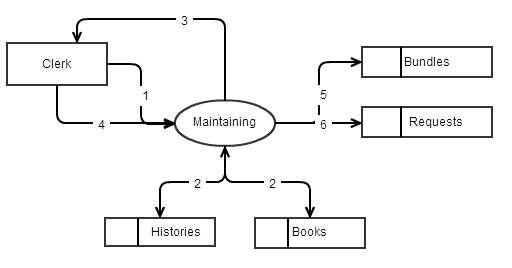
\includegraphics[width=\textwidth]{dfd.png}
            \caption{DFD работы с системой}
            \label{fig:dfd}
        \end{figure}
    \subsection{Система логического вывода}
    \label{sec:logic}
        Предпочтения пользователя описываются с помощью вектора профиля пользователя (см.\,п.~\ref{sec:io}), который
        получается путём нормализации входных векторов начальных предпочтений и истории покупок.

        Профиль конкретного пользователя сравнивается с профилями, которые были определены как тематически"=близкие,
        для того, чтобы определить общие тенденции предпочтений пользователя.
        Таким образом вводится процедура группировки пользователей по критерию похожести профилей.

        В качестве группировки был выбран метод поиска $k$ ближайших соседей.

        Формирование групп позволяет рекомендовать литературу, которая с большой долей вероятности будет интересна
        заданному кругу пользователей.
        Для этого профиль заданного пользователя сравнивается со средними профилями каждой из групп в системе, и
        рекомендуются те книги, которые заданный пользователь ещё не читал.
    \clearpage
\section*{ВЫВОДЫ}
\addcontentsline{toc}{section}{Выводы}
    В рамках этого проекта была исследована экспертная система для рекомендации литературы по информационным
    технологиям для интернет"=магазина книг.
    Она позволяет пользователю найти литературу, которую пользователь ещё не читал и которая бы соответствовала его
    интересам, которые вычисляются согласно предварительному анкетированию и истории покупок/закладок.

    Как показывают исследование разработок рекомендательных систем, подход, рассмотренный в рамках проекта, позволяет
    решить поставленную задачу.
    То, насколько точно будет составлен список рекомендаций напрямую зависит от количества пользователей в системе и
    от их активности.

    В дальнейшем в систему можно добавить возможность автоматического выделения категорий у книги, а также её
    популярности, исходя из доступных в интернете данных.
    \clearpage

\bibliographystyle{ugost2008ls}
% \renewcommand\bibname{Foo}
\bibliography{src}
\clearpage

\begin{landscape}
    \ESKDappendix{}{Дерево решений\label{app:tree}}
    \begin{figure}[h]
        \centering
        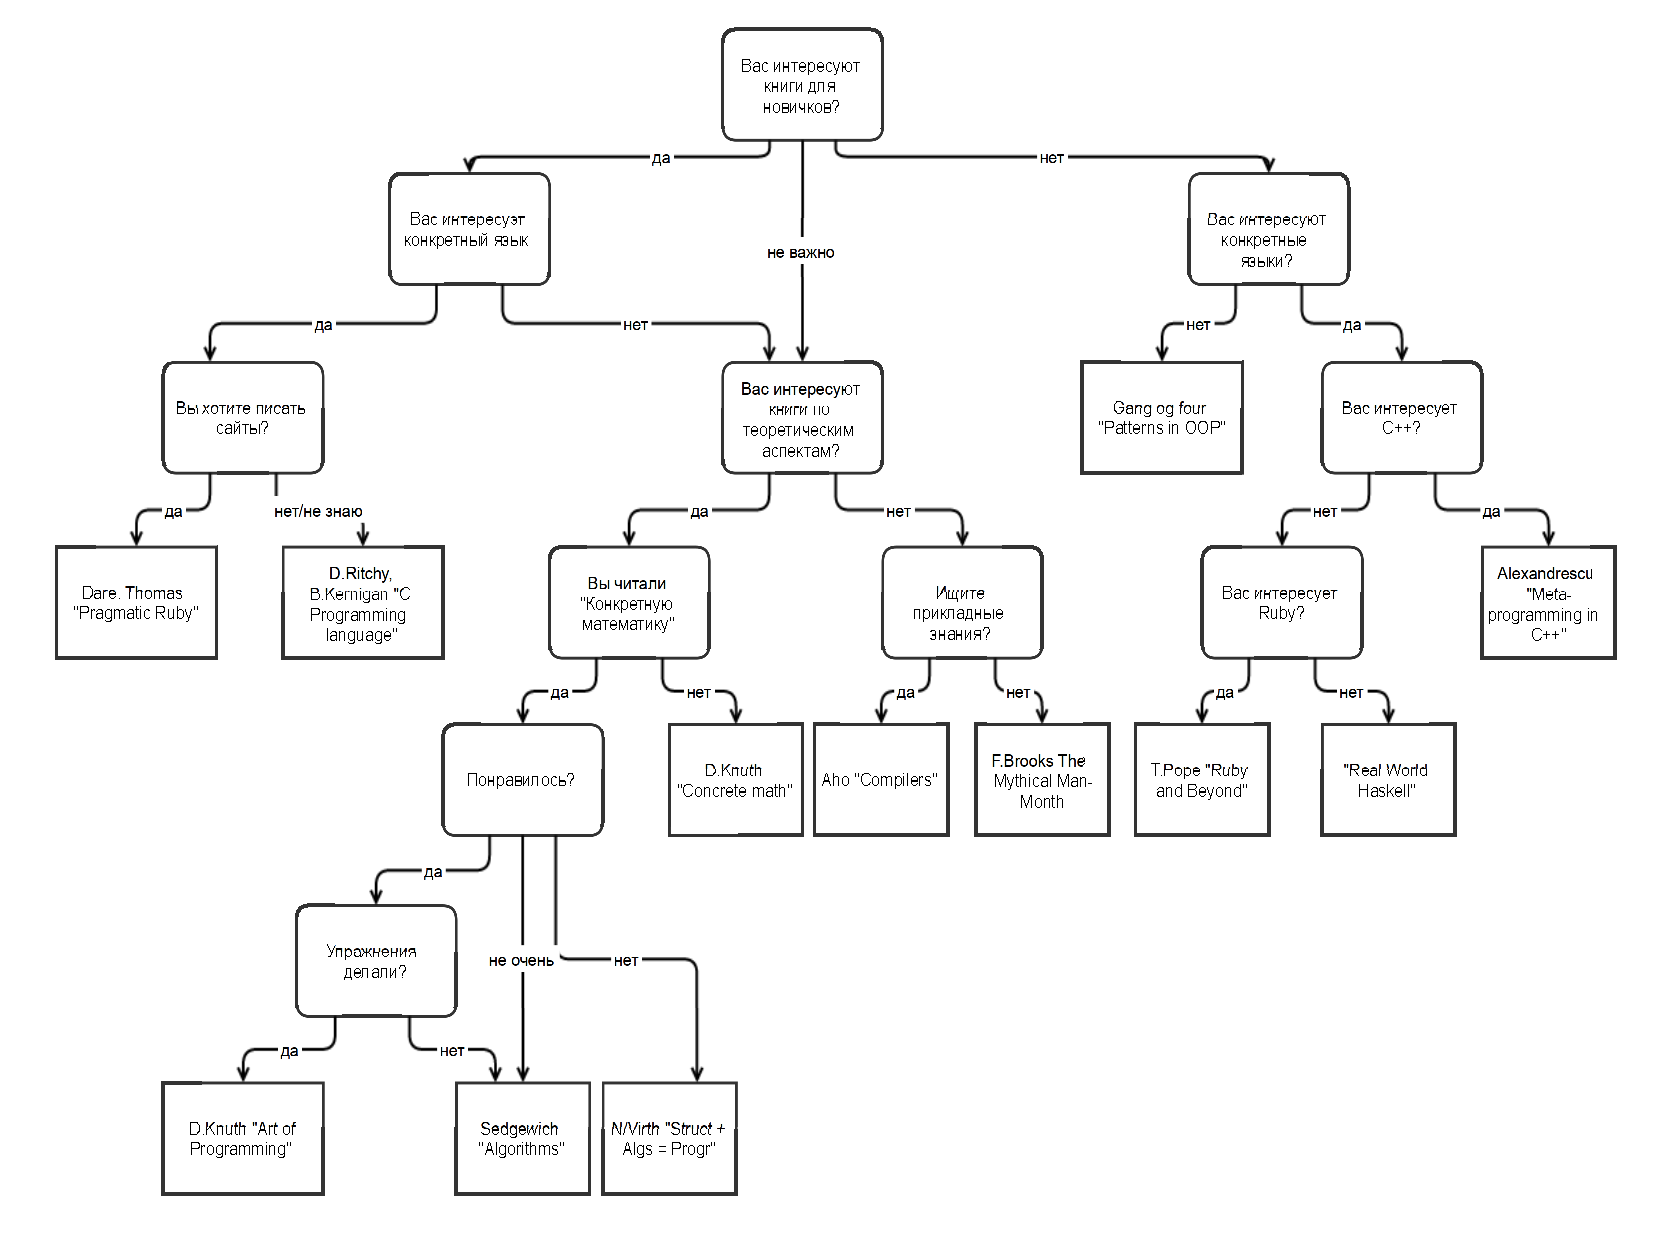
\includegraphics[scale=0.62]{tree.eps}
        \caption{Дерево решений для заполнения начального вектора}
        \label{fig:tree}
    \end{figure}
\end{landscape}
\ESKDappendix{}{Исходные тексты\label{app:sourcecode}}
    \lstinputlisting{../../../compilers_mp/program_stucture.h}
\end{document}
